\documentclass[11pt]{report}
\usepackage[utf8]{inputenc}
\usepackage{csquotes} % Add this line to import the 'csquotes' package
\setcounter{tocdepth}{3}
\setcounter{secnumdepth}{3}
\usepackage{graphicx} % Required for inserting images
\usepackage{appendix}
\usepackage{sectsty}
\usepackage{paperStyle}
\usepackage{tabularx}
\usepackage{siunitx}
\usepackage{tipa}
\usepackage{textcmds}
\usepackage{multirow}
\usepackage{float}
\usepackage[dvipsnames]{xcolor}
\usepackage{soul}
\usepackage[section]{placeins}
\usepackage{pgffor}
\usepackage{amssymb} % for \approx
\definecolor{HLColor}{RGB}{230,230,250}
\sethlcolor{HLColor}
\usepackage[
    backend=biber,
    style=numeric,
    sorting=none
  ]{biblatex}

% TOP MARGIN:
\makeatletter
\setlength{\@fptop}{0pt}
\makeatother

% BIBLIOGRAPHY:
\addbibresource{references.bib}

% TITLE:
\title{\Huge \textbf{Mood Tracker}\vspace{2mm} \\
    \large Part 1: User Interface Design}

% AUTHORS:
\author{\vspace*{1cm}\Large Alexandros Tsaparas
\\ \textit{Supervisor: Christos Sintoris}
\and Electrical and Computer Engineering Department,
\\University of Patras\vspace{5mm} \\
AM: 1072824}
\date{}

\begin{document}
\maketitle 
\tableofcontents

\chapterfont{\LARGE \centering}
\chaptertitlefont{\Large \centering}
\chapter{User research - Key problems}

\section{Introduction to the Mood Tracker app}

In the following, the basic principle of the app is presented in order to be able to better classify all procedures and results of the user research and problem identification in the topic field.\\ \\
The core premise of the application revolves around the identification of issues and concerns through regular anonymous surveys/forms created by the professors and administered to university students. Furthermore, it aims to provide initial ideas and thoughts to improve the overall student environment. The app is specifically designed for universities interested in students satisfaction. Survey results are provided to professors in a completely anonymous format. Students can view their mood history and analyze how their survey answers have changed over time. In addition, there should still be a way for students to contact their supervisors directly to communicate individual ideas and suggestions.\\ \\
Finally, it's worth mentioning that after the first chapter of the report, the features of the app may change or even new ones may be added, as the user research and problem identification may lead to a different direction.

\section{Preparatory Research}

The following item deals with the relevance of my app as well as the user research. In particular, it discusses why student satisfaction is important for universities. For this purpose, various scientific articles and publications as well as contributions from health-related organizations were considered. In addition, a comprehensive analysis of similar apps in the market was undertaken to identify existing features, drawbacks, and potential areas for improvement. This research aimed to uncover missing opportunities for users and explore innovative ideas that could be implemented to enhance the overall user experience. Furthermore, an exemplary survey was conducted in order to be able to specifically address user requirements when designing the app.

\subsection{Relevance of a Moodtracker for Universities}

In the course of my user research, I found numerous sources that prove that student well-being is directly related to their productivity. Numerous universities globally invest resources in understanding the intricate connection between students' mental health, stress levels, and academic performance. Additionally, beyond academia, researchers from various fields explore well-being across demographics, employing diverse methodologies such as surveys and longitudinal studies.

\subsubsection{First research}

\textbf{University of Applied Sciences, Northern Netherlands \cite{research-1}}
\\ \normalsize Taking advantage of the high number of students who study at their institution, they collected data through in-depth and open-ended interviews between May and November 2020 (beginning of the COVID-19 pandemic).\vspace{5mm} \\
\textbf{Method} \\
A total of 113 students signed up for interviews, selected through purposive sampling based on criteria like full-time status, well-being problems, and diverse representation. They were surely informed from researchers (intranet messages) and Heads of School. Participants were from various academies, study years, and genders. Interviews, lasting 28 to 52 minutes, explored student well-being and related factors. Consent was obtained, and interviews were video recorded. The semi-structured guide covered topics such as defining well-being and factors influencing it. Data collection continued until saturation, with 27 students interviewed.\vspace{5mm} \\
\textbf{Analysis} \\
Thematic analysis was used to interpret data, involving verbatim transcription, member checks, and independent coding by three researchers. Coding was initially done line by line using an open coding approach, with the possibility of applying multiple codes to a passage. Codes were then organized into categories based on data and literature concepts, forming themes. Categories, themes, and data allocation were verified in the final phase by two other researchers to ensure clarity and consistency. Discussions resolved any discrepancies until an agreement was reached.\vspace{5mm} \\
\noindent \textbf{Results} \\
Participated five male students, twenty-one female students, and one non-binary student, all aged between 17–24 years, participated. There was revealed a diverse range of self-reported well-being issues among the participating students. These included challenges such as inadequate support from the school, anxiety disorders, family-related issues, physical health problems, symptoms of depression, gender dysphoria, fatigue, and performance anxiety. Additionally, factors like stress, planning difficulties, study pressure, loneliness, perfectionism, and getting used to studying were frequently mentioned by the students. Some participants highlighted the impact of life phase-related problems, ADHD, and drug use on their well-being. The findings underscore the complexity and multifaceted nature of the well-being issues faced by students, emphasizing the need for a holistic approach in addressing these concerns, both within and beyond the academic environment.\vspace{5mm} \\
\textbf{Students' opinions} \\
They expressed diverse views on student well-being. Initially, some found it challenging to define, but as interviews progressed, themes emerged. Well-being was associated with managing stress, achieving balance in academic and personal life, and acknowledging the effort-achievement ratio. Stress and resilience were central themes, with students emphasizing the need to cope with challenges. Well-being was seen as a combination of mental, physical, and social aspects, with support from the university playing a crucial role. Students acknowledged the fluctuating nature of well-being and its significant impact on academic performance.\vspace{5mm} \\
\textbf{Main Factors} \\
The main factors influencing student well-being include self-regulation, perfectionism, motivation levels, ability to plan, and study achievements at the individual level. \underline{Fellow students} contribute to well-being through practical support, idea exchange, enjoyment, and fostering a community atmosphere. \underline{Tutors} play a crucial role with good relationships, trustworthiness, accessibility, and time availability. \underline{Attitudes} and \underline{behaviors} such as empathy, guidance, and personal attention also influence well-being. \underline{Teachers} impact well-being through good relationships, accessibility, informal contact, community atmosphere, and attitudes like reassurance, understanding, and recognition. Study-related factors include clear communication, flexibility, workload, and the scale of education. The \underline{university's} support facilities and community atmosphere are significant. \underline{Peers} outside the university contribute to well-being through enjoyment, idea exchange, understanding, and recognition. \underline{Family} support, idea exchange, and enjoyment are also key factors.

\subsubsection{Second research}

\textbf{Renmin University of China, Haidian, Beijing, China \cite{research-2}}
\\ \normalsize The university conducted research on students' well-being, recognizing the importance of mental health in maintaining overall health. The study addresses the global rise in depression and anxiety cases, particularly among college students. College is identified as a critical period for shaping values, and students' emotional well-being is linked to various factors.\vspace{5mm} \\
\textbf{Method} \\
This study employed data from the "Beijing College Student Panel Survey" within the "China Education Panel Survey," focusing on the 2008 cohort of students tracked for four years from 2009 to 2012. Sampling involved 15 universities, and the effective sample size was 1401 students. The investigation utilized the Depression Anxiety Stress Scales-21 (DASS-21) to assess psychological well-being, a self-report measure known for its reliability. The DASS-21 includes three scales for depression, anxiety, and stress, each comprising seven items. Scores are calculated by summing corresponding item scores. Notably, the DASS-21's short version requires scores to be multiplied by two for comparison with conventional severity ratings. The study reported good validity for the DASS measurement, supported by scale reliability coefficients of 0.813 for depression, 0.766 for anxiety, and 0.812 for stress. Overall, the methodology involved a comprehensive survey approach, online and on-site rounds, and rigorous measures for assessing students' mental health across their college years.\vspace{5mm} \\
\textbf{Results} \\
The results from the study, provide insights into the mental well-being of Chinese college students across four academic years. The average scores for depression and stress, ranging between 7.22 and 7.79 for depression and 9.53 and 11.68 for stress, consistently fell within the normal range based on cutoff values. However, anxiety scores in the first three years slightly surpassed the normal threshold of 7, with mean scores of 7.40, 7.24, and 7.10, indicating above-average anxiety levels. The previously mentioned statistic numbers, as they increase they reflect more and more the severity of depressive and stress-related symptoms. Interestingly, anxiety levels seemed to decrease in the senior year, with a mean score of 6.63. Despite above-normal anxiety levels in the initial years, students maintained mental health with depression and stress scores in the normal range. The study suggests a fluctuation in mental states, with students experiencing higher stress and depression in the sophomore year, while improvements were observed in the last two years. These findings shed light on the dynamic nature of college students' mental well-being over their academic journey, emphasizing the need for targeted interventions and support to enhance mental health throughout their college experience.\vspace{5mm} \\
\textbf{Discussion and Conclusion} \\
In conclusion, the study sheds light on the mental well-being of Chinese college students over four academic years. Freshmen and sophomores exhibited more mental health challenges, possibly stemming from adjustment issues and increased study pressures. Financial concerns were identified as a significant contributor to anxiety, with Chinese students having relatively lower financial burdens compared to their UK counterparts. Notably, the study revealed differences in psychological well-being trends between China and the US, emphasizing the need for tailored interventions. The longitudinal approach strengthened the credibility of the findings, highlighting grade-related disparities. Key conclusions include the average mental health of Chinese college students, their vulnerability to anxiety in the initial years, and the improvement in psychological well-being over time. The study recommends targeted psychological guidance for different academic years, emphasizing the importance of addressing anxiety in freshmen and enhancing well-being support for sophomores. Future research may explore students' mental changes after entering the workforce for further insights into the development of psychological well-being counseling programs in college.

\subsubsection{Third research}

\textbf{Introduction} \\
This article \cite{research-3} delves into using accelerometer data from smartphone keyboard usage to explore connections between typing dynamics, mood, cognition, and daily variations. Focused on a clinical sample, it reveals that individuals with higher cognitive performance show distinct daily patterns in smartphone keyboard use. The study emphasizes the potential of passive smartphone sensor data for monitoring mental health features. It also touches on other accelerometer applications, from wrist-worn devices in clinical populations to predicting sleep patterns. The article discusses the limited use of a sensor fusion approach, combining accelerometer data with keyboard dynamics, and concludes with objectives to analyze daily patterns in data and explore individual differences.\vspace{5mm} \\
\textbf{Method} \\
In a comprehensive study focusing on individuals aged 25 to 50 with mood disorders and healthy controls, researchers employed a multifaceted approach to investigate behavioral biomarkers for mental health. Recruited through community outreach, participants underwent eligibility assessments and exclusion criteria were applied, including acute suicidal ideation and contraindications to MRI. Over four to five weeks, participants used a custom-built smartphone keyboard, BiAfect, exclusively during the study, capturing keystroke dynamics and excluding swiping. Cognitive assessments and mood evaluations were conducted using digital versions of the Trail Making Test Part-B, Quick Inventory of Depressive Symptomatology, and Young Mania Rating Scale. Data processing involved pre-processing keyboard dynamics and accelerometer data, extracting variables such as transition type, inter-key delay, and phone orientation. The study's statistical analyses utilized mixed-effects models, incorporating mood assessments, age, cognitive performance, keyboard dynamics, and demographic variables. The goal was to establish detailed individual behavioral profiles over time, contributing to the development of BiAfect as a tool for collecting dense samples from smartphones and wearables to uncover interconnections between digital behaviors, cognition, mood, and daily activities. Figures were generated to visualize predicted values, emphasizing the interaction between diurnal patterns and cognitive performance. The research aimed to enhance understanding and pave the way for more frequent and nuanced mental health assessments.
\newpage
\noindent \textbf{Results and Conclusion} \\
Focused on individuals with mood disorders and healthy controls, the study revealed lower processing speed and executive functioning in the mood disorder group, even in cases of mild symptom severity, aligning with existing literature on cognitive impairment in non-acute states. The integration of Ecological Momentary Assessment (EMA) data highlighted the interaction between daily patterns and cognitive differences, emphasizing the importance of considering individual variations. While individuals with higher cognitive performance exhibited faster typing and were less affected by time of day, the discussion delves into the potential of passive sensor data for providing nuanced insights, supporting a precision medicine-based approach in behavioral health. While recognizing some limitations, like mild symptoms and using the time of day instead of time since waking up, the study suggests that using smartphones for regular, non-intrusive assessments of brain health is doable. The findings suggest a promising avenue for future research, tapping into the affordability, scalability, and ubiquity of modern smart technologies in advancing my understanding of neurological and psychiatric disorders.

\subsection{Concluding Insights on Student Well-Being in Higher Education}

In distilling insights from diverse university research studies on student well-being, a stark reality surfaces, unveiling the intricate challenges that students in higher education confront. The imperative of adopting a student perspective, as underscored by Douwes et al. \cite{research-1} and Liu et al. \cite{research-2}, emphasizes the urgency of comprehending well-being from the direct vantage point of those immersed in university life. Both investigations expose a disconcerting trend: students' psychological well-being undergoes discernible fluctuations amid the labyrinth of academic expectations, workload pressures, and examination stressors. Furthermore, the incorporation of established scales, such as the Short Warwick-Edinburgh Mental Well-Being Scale and the Perception of Academic Stress Scale, provides an unflinching framework, casting light on the prevailing issues of mental health and academic stress. On the other hand, Emma Ning et al. \cite{research-3} aim to explore the potential of passive smartphone sensor data for monitoring mental health features. It also touches on other accelerometer applications, from wrist-worn devices in clinical populations to predicting sleep patterns. The main goal is to benefit the use of a sensor fusion approach, combining accelerometer data with keyboard dynamics. The article concludes with objectives to analyze diurnal patterns in data and explore individual differences.\\ \\
"The student well-being model" proposed by Soutter et al. \cite{research-4} contributes significantly to the arsenal of tools for gauging student well-being. Drawing from empirical and theoretical research, the authors present a nuanced model considering diverse domains and categories that impact students' well-being. This framework stands as an indispensable instrument for educators, researchers, and policymakers, urging them to recognize and elevate student well-being in educational settings. Conversely, Hascher's \cite{research-5} research on quantitative and qualitative approaches to assess student well-being spotlights a concerning reality: a lack of a specific definition and assessment of well-being in the school context. The study introduces innovative tools, including a multi-faceted well-being questionnaire and emotion diaries, offering a holistic evaluation of well-being in school.\\ \\
These studies collectively underscore the pressing need to confront the unsettling status quo of students' well-being in higher education. The synthesis of empirical evidence and theoretical frameworks lays bare the interconnected nature of factors influencing well-being, spanning academic, emotional, and social dimensions. Strikingly, the research paints a picture where universities and educators appear oblivious or inert to the burgeoning well-being crisis. As educational institutions strive to foster supportive learning environments, the revelations from these studies should serve as a clarion call for substantive interventions and policies aimed at ameliorating the comprehensive well-being of students in higher education.

\subsection{Survey as a Tool for User Research}

My survey should help me identify the problems my application can solve and figure out how I can optimize its design to achieve the best result. I chose to design the survey with both quantitative and qualitative questions, such as rating scales and open-ended inquiries, in order to have a better understanding of the participants' experiences. It also has comprehensive range of questions addressing various aspects of the academic experience, making it well-rounded and insightful.

\subsubsection{Realization of the Survey}

Given the scope of my project, I've limited myself to a small number of participants. Nevertheless, I was able to gain valuable experience from mostly my department colleagues and also from other faculties/universities. The survey was conducted online, using Google Forms, and was distributed via social media. The survey was open for a week, and I received 11 responses. The survey was anonymous, and participants were informed that their responses would be used for research purposes only. The survey was divided into five sections, with a total of 17 questions (12 mandatory and 5 optional).\vspace{5mm} \\
\textbf{Survey Components} \\
The survey's first page [\ref{fig:q1}] introduces the research purpose, expresses gratitude to participants, and underscores the importance of their insights in understanding academic challenges. Clear instructions urge participants to share thoughts confidentially, emphasizing the positive impact on creating a more supportive university experience.\vspace{5mm} \\
The second page [\ref{fig:q2}] is all about collecting basic personal information that aims to discern whether university challenges have a uniform impact on the mood of all students or if specific groups are more susceptible.
\begin{figure}[h!]
    \centering
    \subfloat[First]{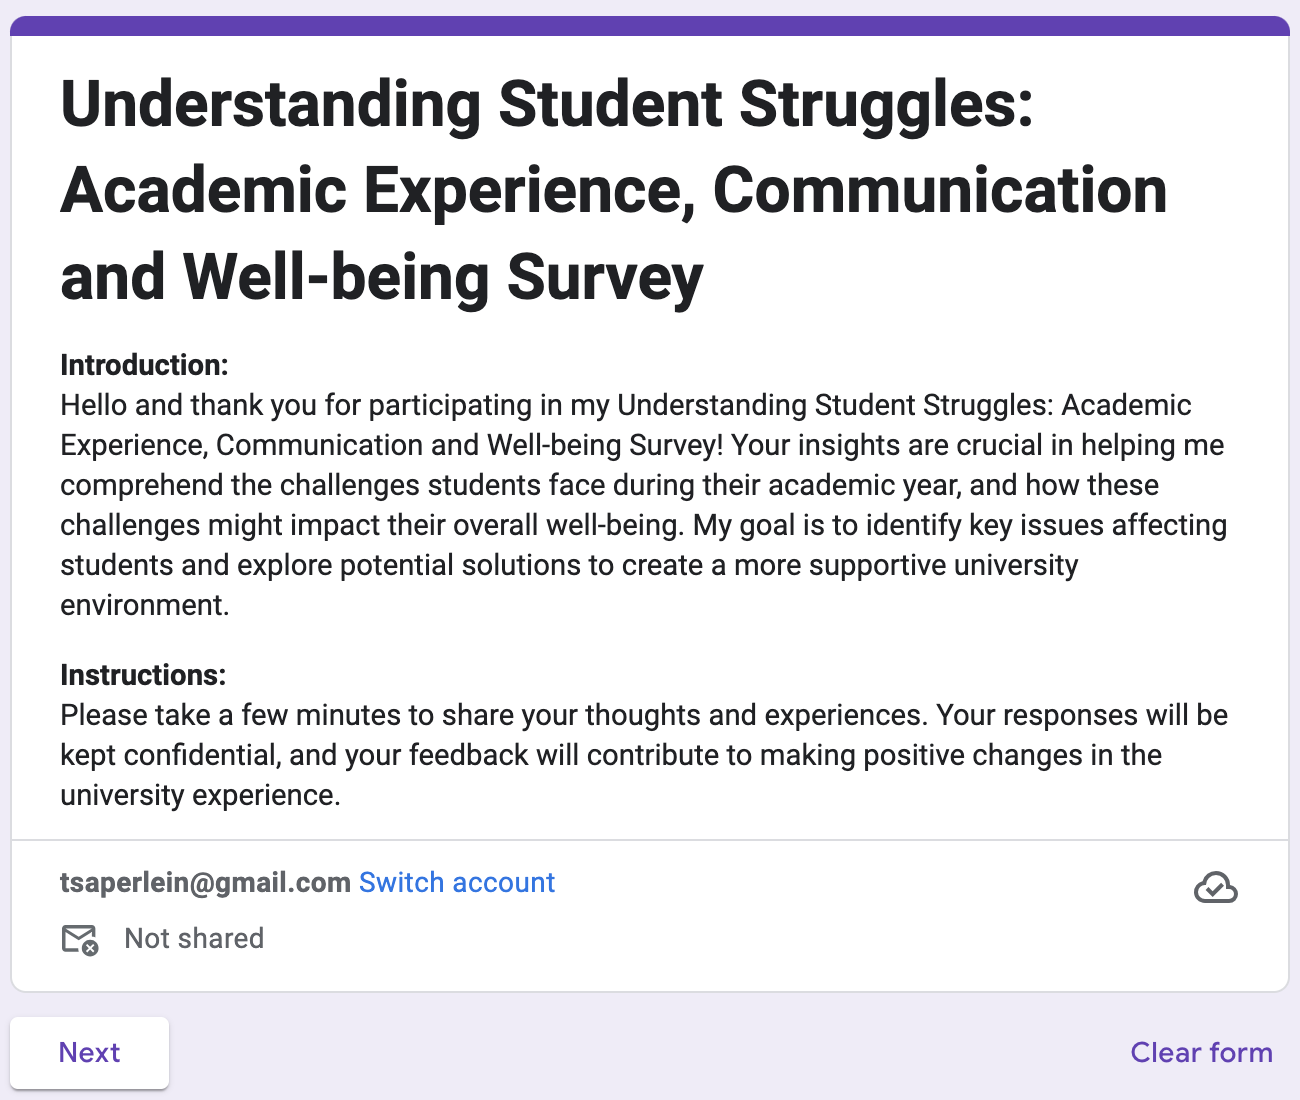
\includegraphics[width=0.52\linewidth]{figures/images/1.png}\label{fig:q1}}
    \hfill
    \subfloat[Second]{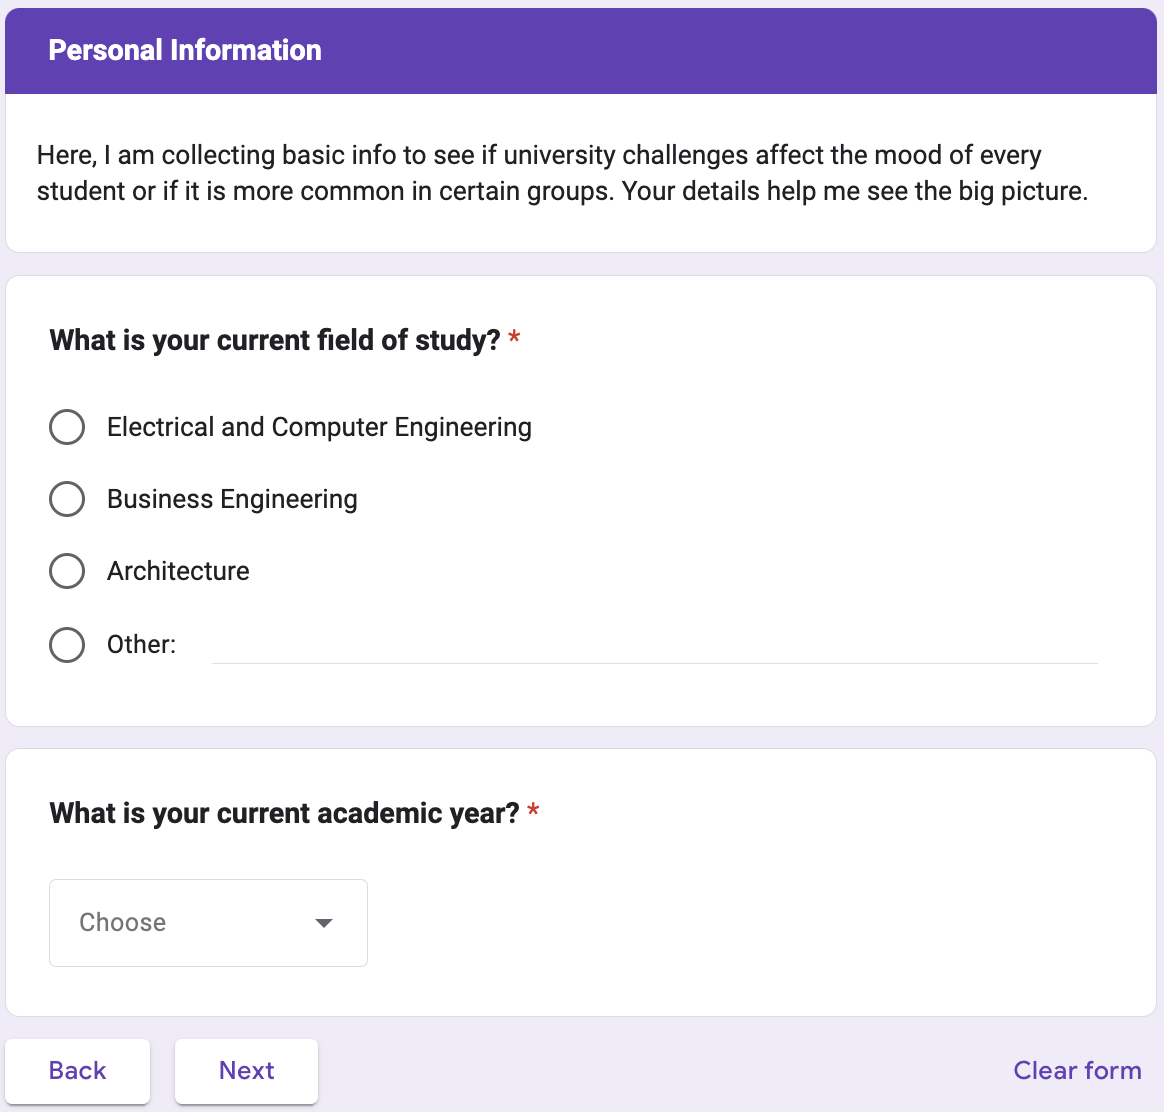
\includegraphics[width=0.46\linewidth]{figures/images/2.png}\label{fig:q2}}
    \caption{First and second page of the survey}
\end{figure} \\
The third page [\ref{fig:q3}] of the survey digs into the academic experiences of participants, by asking a comprehensive set of questions aims to capture nuanced aspects of the academic experience and stressors that contribute to a holistic understanding of the challenges students may face.
\begin{figure}[h!]
    \centering
    \subfloat[Part 1]{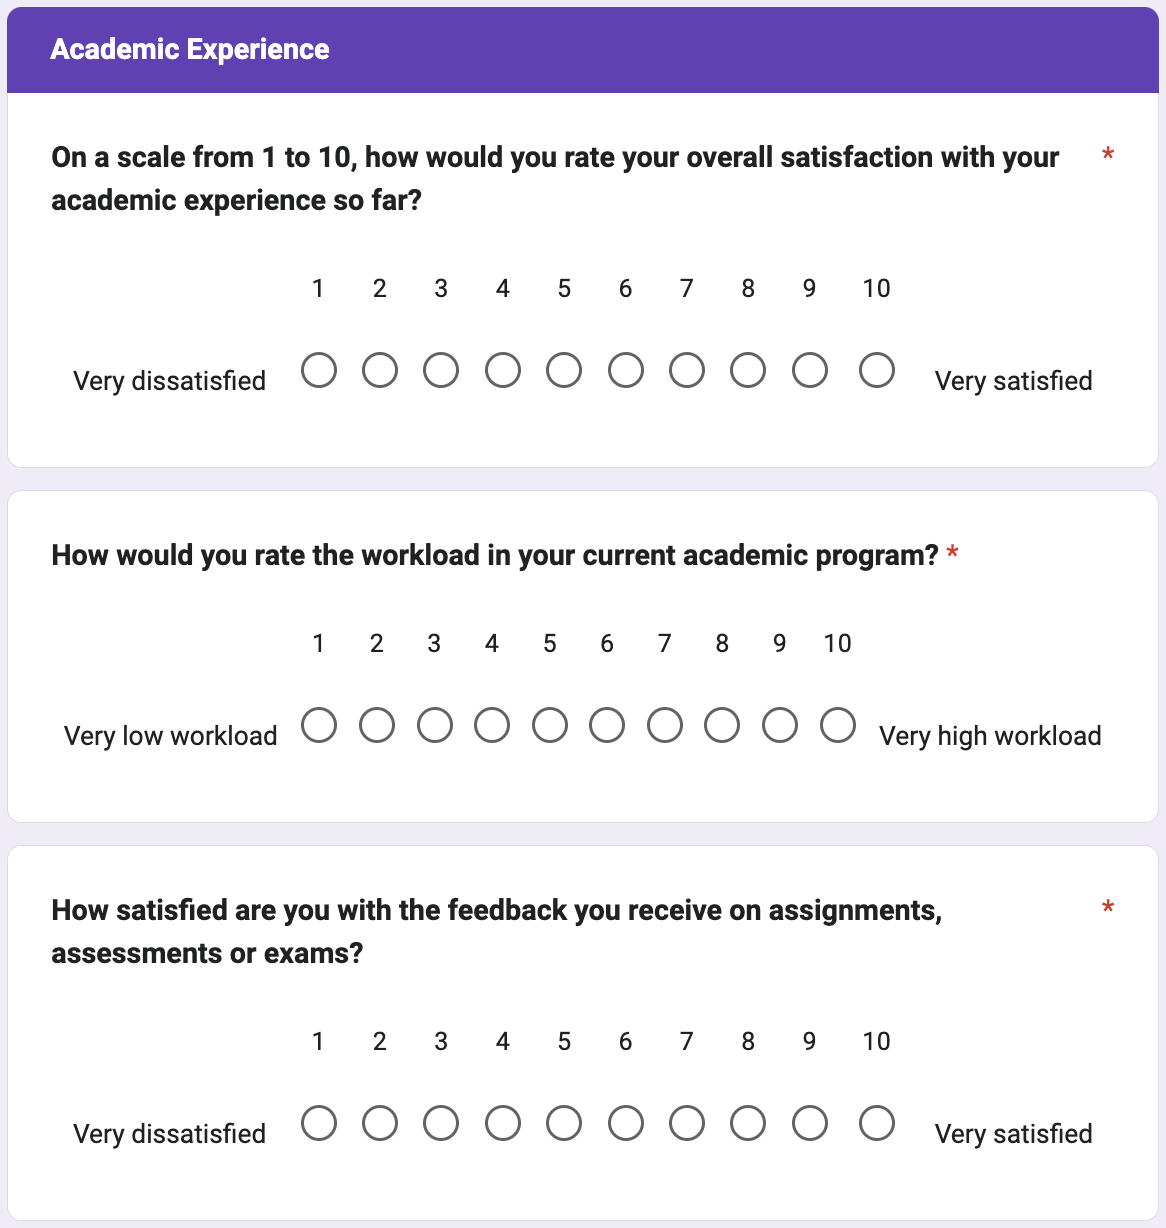
\includegraphics[width=0.49\linewidth]{figures/images/3.png}\label{fig:q3-1}}
    \hfill
    \subfloat[Part 2]{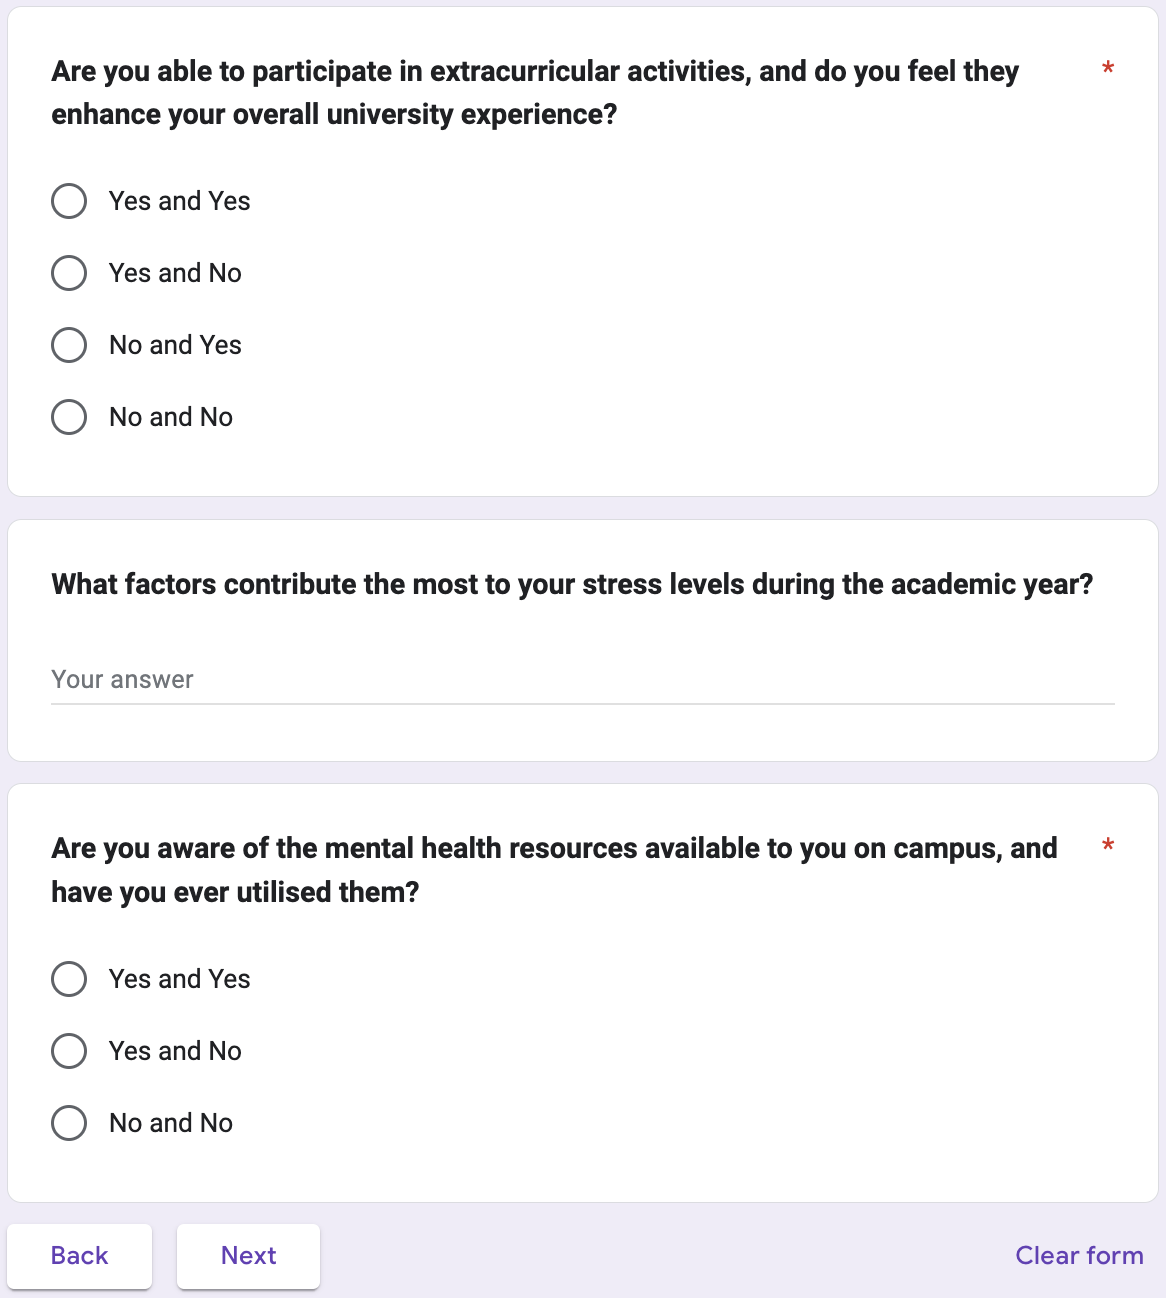
\includegraphics[width=0.46\linewidth]{figures/images/4.png}\label{fig:q3-2}}
    \caption{Third page of the survey}
    \label{fig:q3}
\end{figure}
\FloatBarrier
\noindent The fourth page [\ref{fig:q4}] of the survey focuses on communication dynamics between students and professors. This section aims to uncover insights into the current state of communication between students and professors, allowing for a more detailed understanding of the communication challenges that may impact students' well-being.
\begin{figure}[h!]
    \centering
    \subfloat[Part 1]{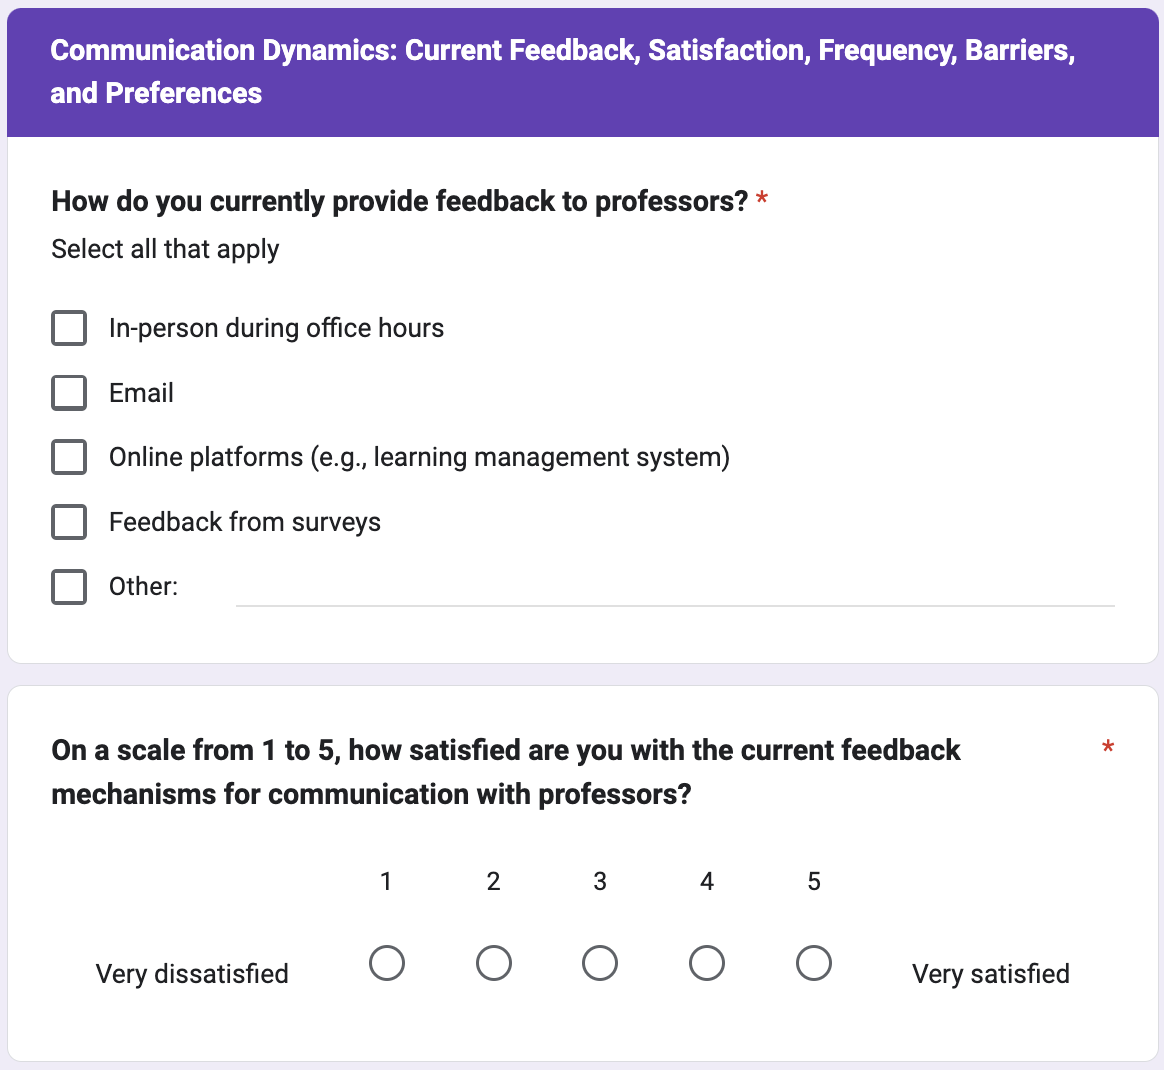
\includegraphics[width=0.48\linewidth]{figures/images/5.png}\label{fig:q4-1}}
    \hfill
    \subfloat[Part 2]{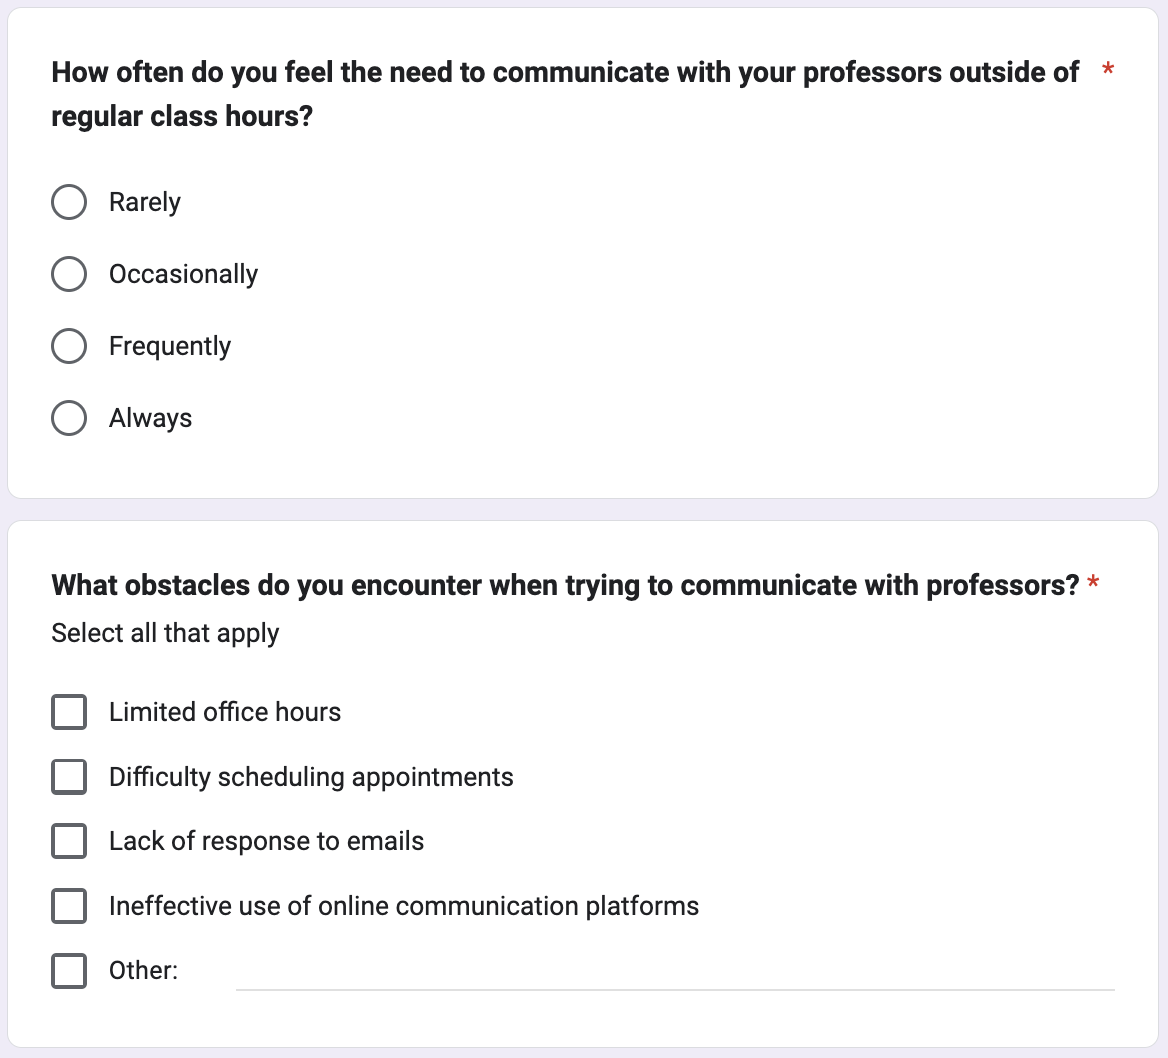
\includegraphics[width=0.49\linewidth]{figures/images/6.png}\label{fig:q4-2}}
\end{figure}
\begin{figure}[h!]\ContinuedFloat
    \centering
    \subfloat[Part 3]{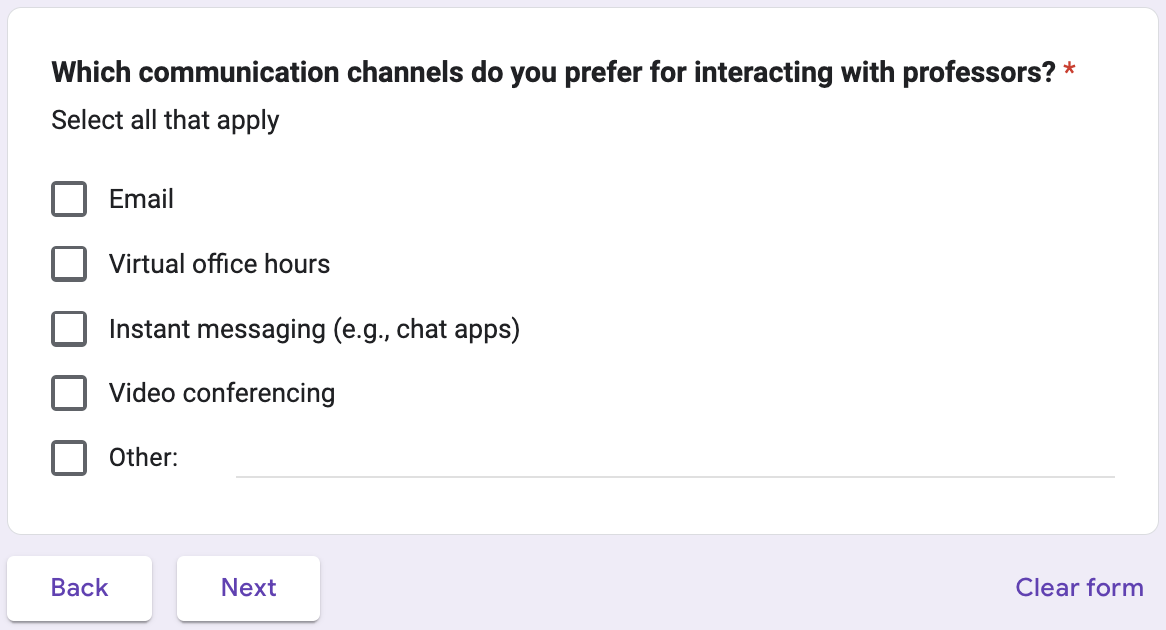
\includegraphics[width=0.49\linewidth]{figures/images/7.png}\label{fig:q4-3}}
    \caption{Fourth page of the survey}
    \label{fig:q4}
\end{figure}
\FloatBarrier
\noindent The fifth page [\ref{fig:q5}] of the survey provides a valuable opportunity for participants to share their insights and contribute to the identification of actionable strategies for creating a more enriching and supportive academic environment.\vspace{5mm} \\
The sixth and final page [\ref{fig:q6}] of the survey gives participants the opportunity to share any additional thoughts or concerns they may have.
\begin{figure}[h!]
    \centering
    \subfloat[Fifth]{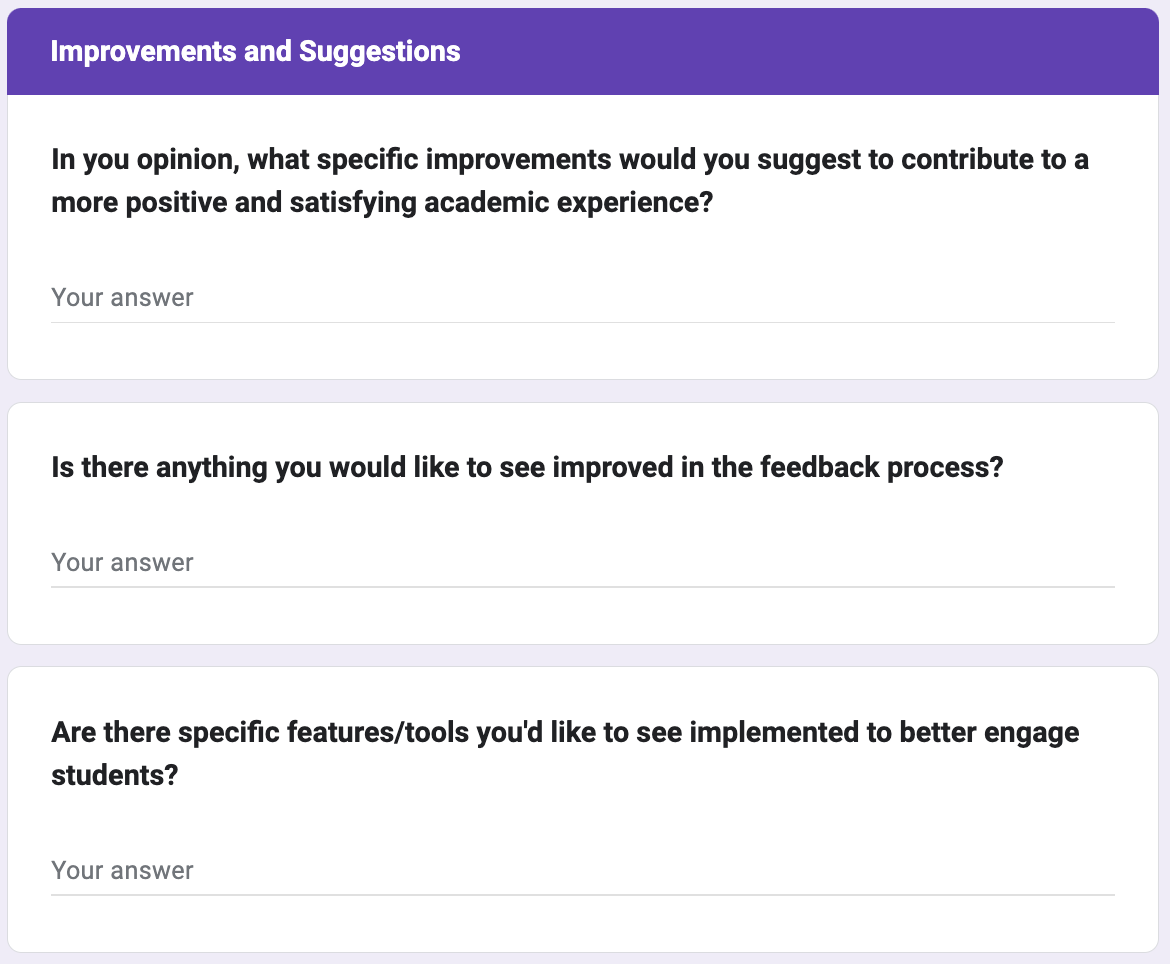
\includegraphics[width=0.46\linewidth]{figures/images/8.png}\label{fig:q5}}
    \hfill
    \subfloat[Sixth]{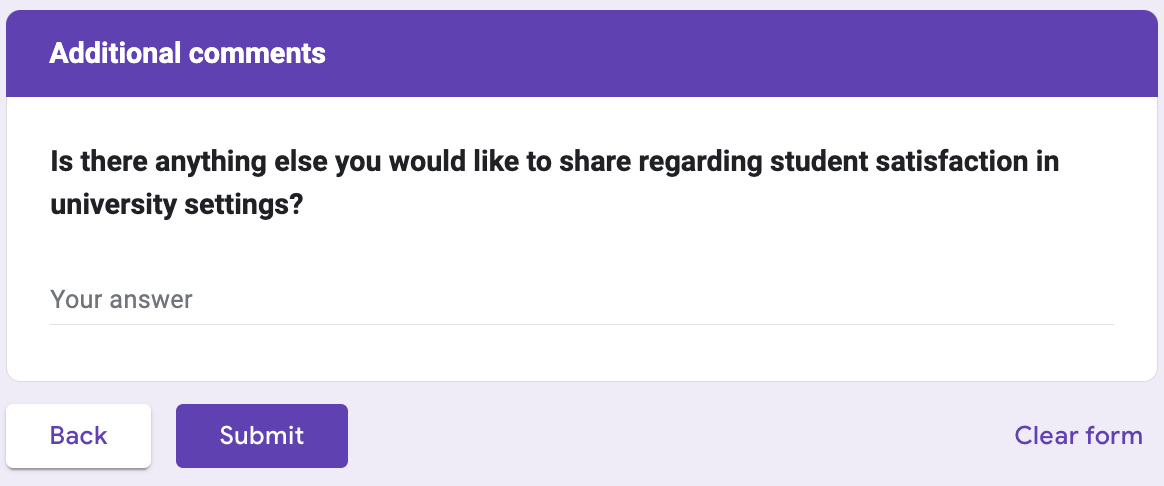
\includegraphics[width=0.50\linewidth]{figures/images/9.png}\label{fig:q6}}
    \caption{Fifth and sixth page of the survey}
\end{figure}

\subsubsection{Results of the Survey}

The results of the survey are presented in the following accompanied by a brief analysis of the findings.
% ----- Personal information
\begin{figure}
    \centering
    \subfloat[]{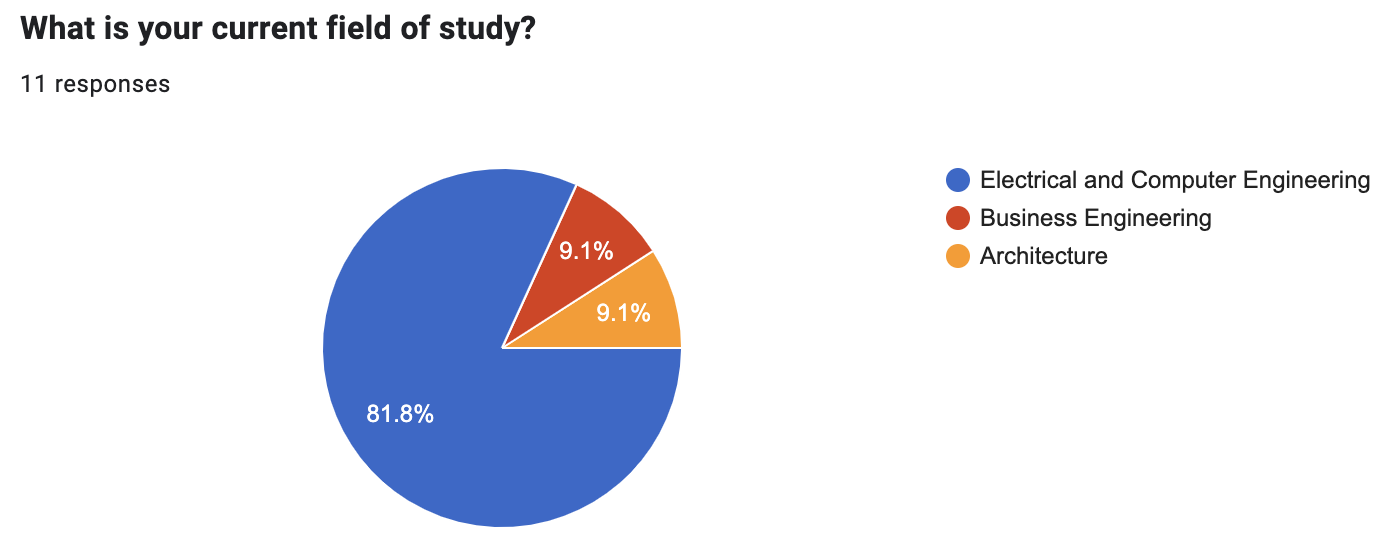
\includegraphics[width=0.9\linewidth]{figures/results/q1.png}\label{fig:q1-result}}
\end{figure}

\begin{figure}\ContinuedFloat
    \centering
    \subfloat[]{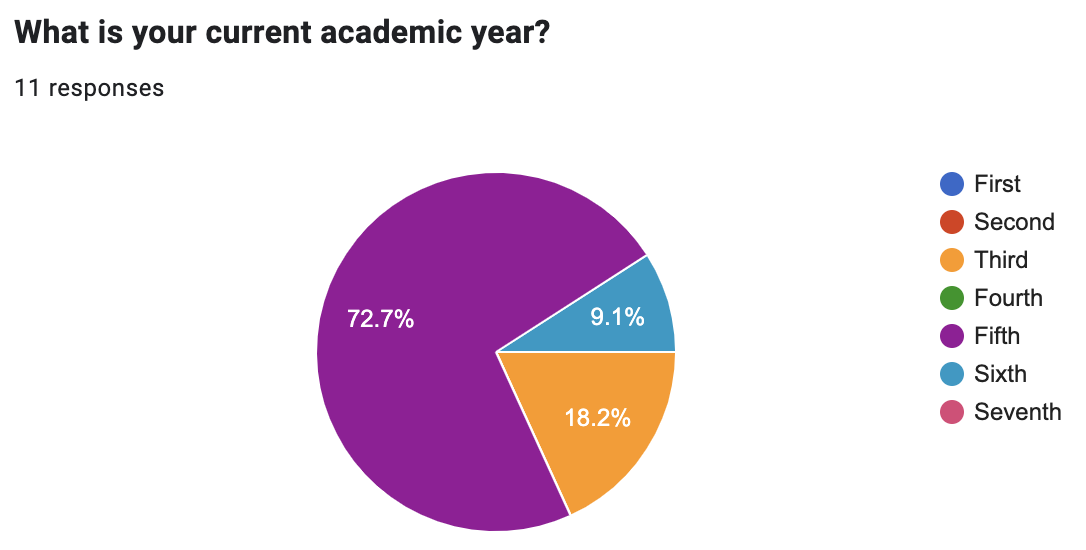
\includegraphics[width=0.9\linewidth]{figures/results/q2.png}\label{fig:q2-result}}
    \caption{Personal information}
\end{figure}

% ----- Academic experience

\foreach \i in {3,4,5,6,7,8}{
    \ifnum\i=3
        \begin{figure}
            \centering
            \subfloat[]{\includegraphics[width=0.9\linewidth]{figures/results/q\i.png}\label{fig:q\i-result}}
        \end{figure}
    \else
        \begin{figure}\ContinuedFloat
            \centering
            \subfloat[]{\includegraphics[width=0.9\linewidth]{figures/results/q\i.png}\label{fig:q\i-result}}
            \ifnum\i=8
                \caption{Academic experience}
            \fi
        \end{figure}
    \fi
}

% ----- Communication Dynamics

\begin{figure}
    \centering
    \subfloat[]{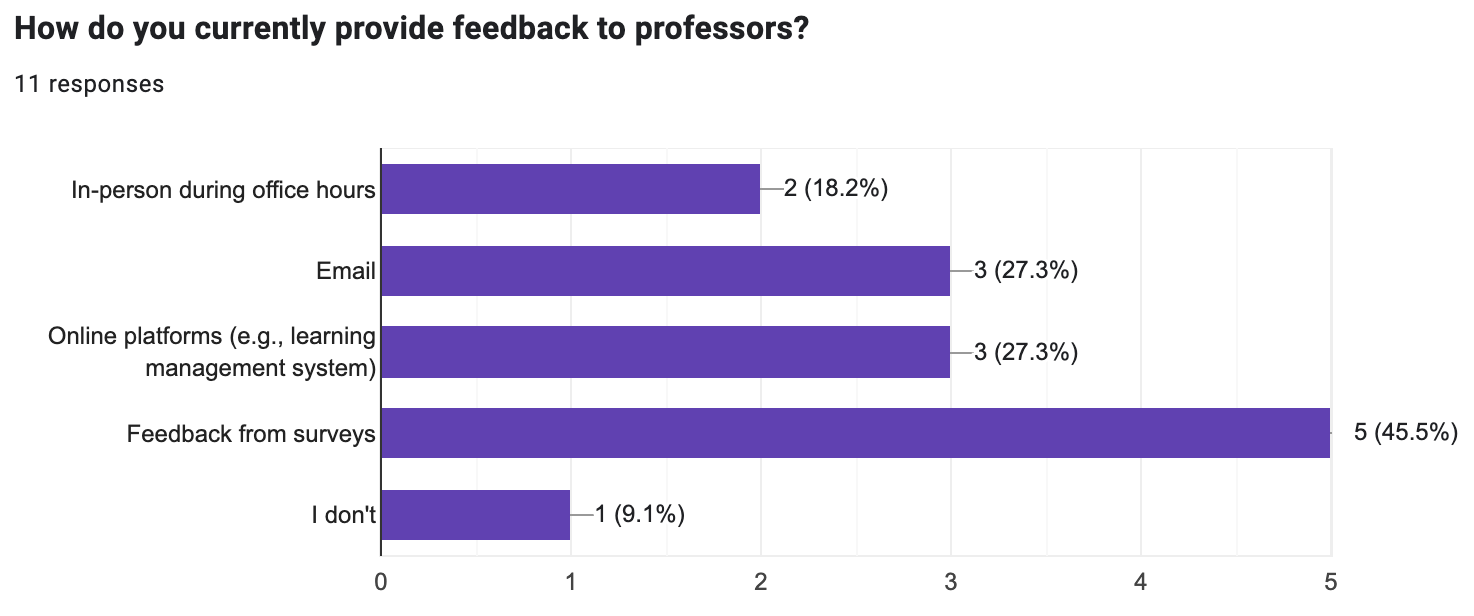
\includegraphics[width=0.9\linewidth]{figures/results/q9.png}\label{fig:q9-result}}
\end{figure}

\foreach \i in {10,11,12,13}{
    \begin{figure}\ContinuedFloat
        \centering
        \subfloat[]{\includegraphics[width=0.9\linewidth]{figures/results/q\i.png}\label{fig:q\i-result}}
        \ifnum\i=13
            \caption{Communication Dynamics}
        \fi
    \end{figure}
}

% ----- Improvements and Suggestions
\begin{figure}
    \centering
    \subfloat[]{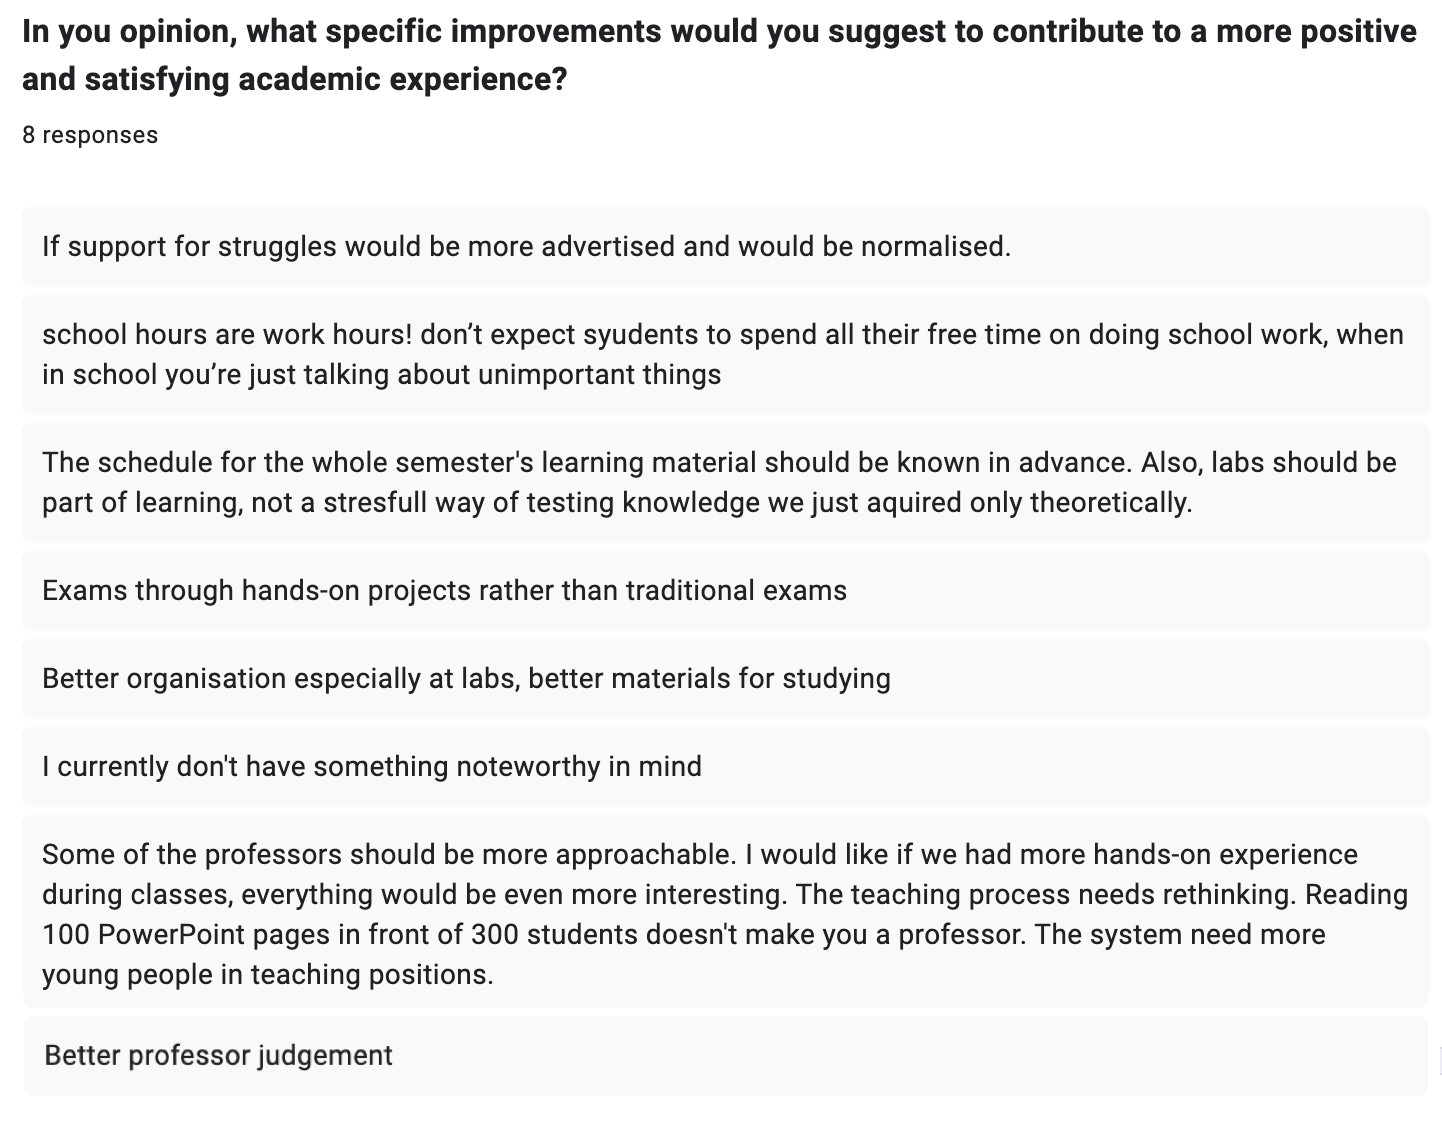
\includegraphics[width=0.9\linewidth]{figures/results/q14.png}\label{fig:q14-result}}
    \caption{Improvements and Suggestions}
\end{figure}

\foreach \i in {15,16}{
    \begin{figure}\ContinuedFloat
        \centering
        \subfloat[]{\includegraphics[width=0.9\linewidth]{figures/results/q\i.png}\label{fig:q\i-result}}
        \ifnum\i=16
            \caption{Improvements and Suggestions}
        \fi
    \end{figure}
}

% ----- Additional Thoughts
\begin{figure}[htpb]
    \centering
    \subfloat[]{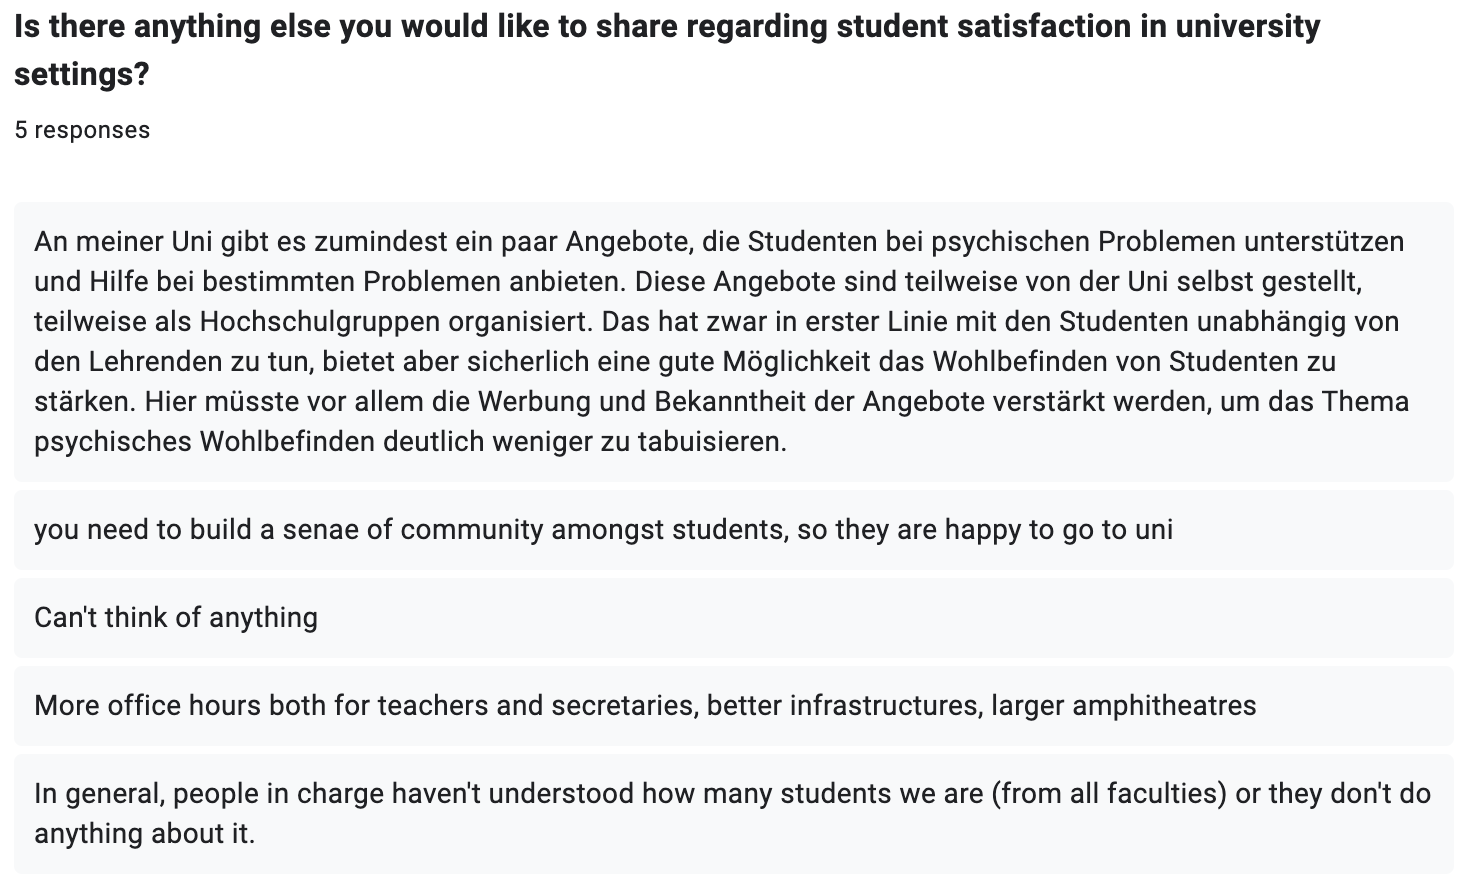
\includegraphics[width=0.9\linewidth]{figures/results/q17.png}\label{fig:q17-result}}
    \caption{Additional Thoughts}
\end{figure}
\FloatBarrier
\noindent \textbf{Field and Year of Study of the participants} \\
The majority of participants are enrolled in Electrical and Computer Engineering indicating a strong representation in this field. Business Engineering and Architecture each constitute of the respondents, showcasing a diverse academic landscape within the surveyed population. Also the fifth academic year is predominant, followed by the third and the sixth years. This distribution may suggest a concentration of survey participants in the latter stages of their academic journey.\vspace{5mm} \\
\textbf{Academic Experience} \\
A considerable number of respondents ($\approx$ 5/10 people) reported a satisfaction rating of 7/10 for their overall academic experience, while approximately 3/10 people reported a rating of 5/10, which means that they are neither satisfied nor dissatisfied. The bulk of participants also considered the workload to be quite substantial, with roughly 5/10 individuals rating it as an 8/10, highlighting the considerable challenges students face in managing their academic responsibilities. We can also observe that most people, around 8/10, take part in after-school activities, and they believe these activities are beneficial. This indicates that being involved in these extra activities not only helps with their studies but also supports overall personal growth. Additionally, 5 out of 10 people expressed dissatisfaction with the feedback mechanisms for communication with professors, indicating potential areas for improvement in this aspect.\\ \\
Notably, a significant proportion of respondents ($\approx$ 9/10 people) identified limited office hours and cited a lack of response to emails as obstacles when trying to communicate with professors. Furthermore, the survey brought to light that  of students are not aware of or have not utilized mental health resources on campus, emphasizing the importance of enhancing awareness and accessibility to support services for the well-being of students. Furthermore, near half of the participants ($\approx$ 4/10 people) reported low numbers about the feedback they receive from their professors about assignments, assessments, and exams, underscoring the need for more comprehensive feedback mechanisms to support students' academic growth and development. According to the contestands, academic stress stems from diverse sources, including the pressure of exams, particularly retakes, heavy workloads, simultaneous deadlines for exams and projects, uncertainties about the future and chosen fields, and concerns about study methods.\vspace{5mm} \\
\textbf{Communication Dynamics} \\
The survey data highlights a significant reliance on feedback from surveys among students, with approximately 5/10 indicating a preference for this communication method over email, online platforms, and in-person office hours. However, despite this preference, half of the students express dissatisfaction with the current feedback mechanisms for communication with professors. This apparent contradiction suggests that while surveys may be a commonly used tool, there might be room for improvement in the effectiveness and responsiveness of the feedback channels.\\ \\
Furthermore, the data indicates a concerning trend regarding student-professor interaction. A majority of students ($\approx$ 8/10) do not feel the need to communicate with their professors, attributing it to a lack of connection. This lack of connection may be influenced by factors such as limited office hours (voted by 10 out of 11 students) and a perceived lack of response to emails ($\approx$ 8/10). The overwhelming use of email as the primary mode of communication ($\approx$ 9/10) suggests that despite its prevalence, students may be facing challenges in establishing meaningful connections and receiving timely support from their professors. Addressing these issues could potentially enhance student engagement and overall satisfaction with the communication channels.\vspace{5mm} \\
\textbf{Improvements and Suggestions} \\
The students provided insightful suggestions for improving their academic experience. A common theme is the need for better support and the normalization of struggles. Students expressed a desire for more advertised support systems and a less stressful environment, suggesting that school hours should be treated as work hours, allowing for a balance between academic and personal time. Another prevalent suggestion is for more transparency in scheduling and a shift towards hands-on learning, with exams conducted through projects rather than traditional methods. Students also emphasized the importance of better organization, materials, and professor approachability, with a call for a rethinking of the teaching process, including more hands-on experiences and the incorporation of young educators. In terms of feedback, students advocated for more active participation and consideration of survey results, hoping for a systematic and regular feedback process that leads to tangible improvements. Lastly, they suggested the implementation of features such as more frequent feedback, increased use of existing tools like Zoom and Skype, and availability of online office hours through apps for better student engagement. These suggestions collectively highlight the students' desire for a more supportive, practical, and engaging academic environment.\vspace{5mm} \\
\textbf{Translated Text from German in [\ref{fig:q17-result}]} \\
\textit{"At my university there are at least a few offers that support students with mental health problems and offer help with certain problems. Some of these offers are provided by the university itself and some are organized as university groups. Although this primarily has to do with the students independently of the teachers, it certainly offers a good opportunity to strengthen the well-being of students. Above all, the advertising and awareness of the offers would have to be increased in order to make the topic of mental well-being much less taboo."} \vspace{5mm} \\
\textbf{Additional Thoughts} \\
The students express a variety of perspectives on their satisfaction with university settings. One student appreciates the mental health support services available at their university, emphasizing the importance of raising awareness to destigmatize discussions around well-being. Another underscores the need to foster a sense of community among students to enhance their overall happiness in the university environment. On the other hand, some students highlight practical concerns, such as the desire for more office hours for both teachers and secretaries, improved infrastructure, and larger amphitheatres. Additionally, there is a shared sentiment that the university authorities may not fully grasp the challenges faced by the student body, whether in terms of their numbers or the need for responsive actions. These diverse perspectives shed light on various dimensions of student satisfaction, from mental health support to community building and infrastructure improvements, suggesting that a holistic approach is necessary for an optimal university experience.

\section{Comparative Analysis of Existing Mood-Tracking Apps}

In my exploration of the most used mood-tracking apps of 2023, I encountered several noteworthy options with distinct strengths and weaknesses. \textbf{\href{https://www.getmoodfit.com/}{Moodfit}}, while lacking in consistency in interface appeal, presents valuable features such as charts and meditation exercises that could enrich the user experience in my app. Slow app, missing some important features and needs more private content \cite{moodfit-review}. \textbf{\href{https://worrywatch.com/}{Worry Watch}}, though limited to iOS and featuring a challenging interface, offers positive affirmations—an aspect that could inspire a focus on mental well-being in my application. Also offers exercises (breathing, meditation) with a variety of options/modifications that create a safe place for the user \cite{worrywatch-review}. \textbf{\href{https://www.moodtools.org/}{MoodTools}}, while maintaining a simple design, could benefit from a more refined frontend and interactive elements, which my app aims to incorporate for enhanced engagement \cite{moodtools-review}. \textbf{\href{https://mobile.va.gov/app/ptsd-coach}{PTSD Coach}}, tailored for military service members, showcases an appealing interface and color palette, influencing my consideration for a visually pleasing design. \textbf{\href{https://emoodtracker.com/}{eMoods (Bipolar Mood Tracker)}}'s complex interface and subscription-based full version might prompt my app to emphasize user-friendly design and affordability. Also is a more specialized app, specific to bipolar disorder (hence the name) \cite{emoods-review}. \textbf{\href{https://www.thriveport.com/products/moodkit/}{MoodKit}}, despite its outdated interface, provides password-protected journals and charts, influencing my app's focus on security and comprehensive mood tracking \cite{moodkit-review}. \textbf{\href{https://daylio.net/}{Daylio}}'s simplicity and color scheme align with my app's objectives, while its inclusion of emoji answers could inspire a similar interactive approach \cite{daylio-review}. The innovative ideas and features inspired by these standout applications will be skillfully integrated, promising users a heightened and more enriching experience.

\section{Key Problems}

Possible key problems with my app are presented and explained in detail below. The problems were categorized into problems that should be solved by future design and problems that arise through human-computer interaction.

\subsection{Problems to be Solved by Future Design}

\begin{description}

    \item[Credibility] The trustworthiness of users in the application poses a potential challenge. Specifically, the anonymization of data might instigate concern among users, as they cannot ascertain whether the data has been anonymized accurately. The ambiguity surrounding the possibility of tracing back information in case of negative feedback from a student could lead to inflated survey results, painting a more favorable picture than the actual reality.
    
    \item[Honesty/Seriousness] Another issue may arise in the manner users approach surveys. There is a possibility that some users may not approach the surveys earnestly, providing inaccurate responses or withholding information when facing challenges with assessments, exams, or professors.
    
    \item[Visualization of the Survey Results] A critical consideration is the effective presentation of survey results. Ensuring results are easily comprehensible and transparent is essential, with a careful approach to prevent distortion based on the presentation method. 
    
    \item[Questions and Answers] The nature of the questions also presents a challenge. Various data collection methods, such as multiple-choice, single-choice, sliders, or grading scales to gauge agreement with a statement, offer diverse avenues. Particularly with the latter, it's crucial to recognize that responses might carry inherent biases. For instance, on a grading scale, users may tend towards more favorable ratings. Consequently, selecting answer options in sentiment surveys demands meticulous attention. 
    
    \item[Application Constraints] Beyond the aforementioned concerns, it's imperative to acknowledge the inherent limitations of the application. Personal issues affecting students outside the university realm may be intricate and go beyond the scope of the app's capabilities. Identifying such problems and providing meaningful assistance in finding solutions can be challenging for the application.
    
\end{description}

\subsection{Possible HCI Problems}

\begin{description}
    
    \item[Simplicity of the App] The app's design should embrace simplicity, ensuring that users are not inundated with complexity, enabling easy comprehension and utilization. If the application's structure becomes overly intricate, there is a possibility of user impatience leading to app abandonment or even deletion.

    \item[Persuasion Dilemma] A primary objective in design is to craft the application in a manner that persuades users to place trust in its functionality and engage with it sincerely. The elements discussed under "Trustworthiness" and "Veracity/ Credibility" earlier encapsulate precisely this objective.

    \item[Information Visualization Challenge] Effectively presenting information poses a common challenge. This is exemplified in the aforementioned points concerning the "Visualization of the Survey Results" and "Questions and Answers." Striking the right balance is crucial, ensuring that users are not overwhelmed by excessive information while providing a comprehensive overview of the most crucial details.
    
\end{description}

\section{Conclusion}

Building upon the insights gathered from the aforementioned articles on students' moods in universities and my comprehensive survey aimed at uncovering the most pressing issues affecting their well-being, my mood-tracking application takes a pioneering approach. The information gleaned from these sources has been instrumental in shaping a solution that not only combines the best features from existing apps but also digs into the core challenges faced by students in the university environment.
\newline

The combination of these sources has enabled my application to transcend the limitations observed in current solutions. It aims to provide an unparalleled, user-friendly experience that not only visually captivates users but also serves as a powerful tool for understanding and anonymously tracking students' moods efficiently. My solution is not merely an integration of features; it is a thoughtful response to the intricate interplay of factors influencing the emotional landscape of students in higher education.
\newline

Moreover, students generally perceive the academic demands as notably intense and burdensome. This insight underscores the demanding nature of the academic experience, where students grapple with a rigorous curriculum, facing significant hurdles in their pursuit of academic success.


\chapterfont{\LARGE \centering}
\chaptertitlefont{\Large \centering}
\chapter{Scenarios - Model of future solution - Paper Mockups}

\section{Scenarios}

\subsection{Scenario 1}

Ioannis is a student in the faculty of Electrical and Computer Engineering in the University of Patras. He is currently in the middle of the winter semester, so he has to work on projects and also start preparing for the final exams. One of his teachers, ms. Sotiriou, has decided that the completion of her course "Advanced Cybersecurity Protocols and Practices" can be achieved by attending the tutorials, completing a project during the semester and also taking tests every week. Although Ioannis is one of the top students in his class/year, he struggles with all the compulsory work of the previously mentioned course and takes more time working on it than other courses. One day, during a break, he tries to talk to his classmates/colleagues about the situation, in which they express the same opinion/struggle. Mutually they decide to talk to the teacher about the exhausting way of evauating their performance in her course. To their surprise, the teacher understands the situation, but decides to stick with the current procedure thinking that only a small amount of students can't cope with it. The student eventually gave up trying to persuade their teacher.
\newline

\noindent Then Kostas, one of Ioannis colleagues, proposed a new app called "MoodTrackU" that will help them with their problem. They suggest the app to their fellow students and also to their teachers. After one day of usage, ms. Sotiriou saw that her course "Advanced Cybersecurity Protocols and Practices" had the most negative feedback comparing to her other courses. Realizing the seriousness of the situation she deicdes to take corresponding actions, such as reducing the amount of tests from one per week to one per three weeks. In the end, the students were satisfied with the result and subsequently realized the potential of the app.

\subsection{Scenario 2}

Mr. Bruck is a professor in California Institute of Technology (Caltech) and he is currently teaching the course "Computation \& Neural Sys" a core course in the factulty of Engineering \& Applied Science. Since the semester is already half over the teacher witnesses frustation and dissatisfaction from the students' side. The teacher doesn't understand the reason behind their behavior, so he tries to contact with them during one of his lectures, by asking for feedback. To his surprise the class doesn't express any discomfort/concern, so he doesn't know what to do.
\newline

\noindent Some days later, mr. Bruck comes accross a mobile app called "MoodTrackU" that helps students and teachers have better communication in universities, by tracking their mood and sending anonymous feedback to the teachers. So he decides the next day to propose the new app to the students in order to understand if there is a problem, or the students are just scared/embarrassed to say their concern about the course. Surprised again, he got a totally different feedback this time, with the students expresssing their problems with his course. After that, he decided to reduce the workload of the semester project and also explain the tasks thoroughly. In the end, the students were satisfied and also successful in passing the course with top grades.

\subsection{Scenario 3}

Inside the St. Augustine’s College, Lily and her peers found themselves overwhelmed by the demands of Professor Bennett's "Advanced Physics" course. Despite voicing their concerns directly to him, his steadfastness remained unchanged. Turning to a new app they found, called "MoodTrackU", which reveals their collective dissatisfaction, they hoped for change, but Bennett's response fell short.
\newline

\noindent Their dissatisfaction continued and as the days passed, the app suggested the students to talk to a higher teacher/person inside the school. So the students turned to the principal, by fully informing him about the situation. She decided to take some actions about it, so she lectured the teacher about his behavior and also his future position to the school. After that, the teacher listened to the students demands and they found a common solution, that benefits both sides. 

\section{Storyboards}



\section{Hierarchical Task Analysis}

\subsection{Plans}

\paragraph{First:}\mbox{}\\
1. Create a new survey:
\newline
1.2.1 $\rightarrow$ 1.2.2.1.1 $\rightarrow$ 1.2.2.1.2
\newline

\noindent 2. See the results of the survey:
\newline
1.3.1 (latest survey) or 1.3.2 (previous surveys)
\newline
$\rightarrow$ if action has been done, do 1.4
\newline

\noindent 3. Create a new team: 1.1.1.1 $\rightarrow$ 1.1.2.2 
 
\paragraph{Second:}\mbox{}\\
1. Answer the survey: 2.2.1 $\rightarrow$ optional: 2.2.2
\newline
\noindent 2. Get suggestions to improve the mood: 2.1.3

\paragraph{Third:}\mbox{}\\
Log in: If there is already an account, do 3.2
\newline else: 3.1.1 $\rightarrow$ 3.1.2 $\rightarrow$ 3.1.3

\section{Paper Mockups}

\subsection{Design Studio}

\subsection{Final Mockup}

\chapterfont{\LARGE \centering}
\chaptertitlefont{\Large \centering}
\chapter{Creation and Evaluation of  Lo-Fi prototype}

\section{Introduction}

\section{Prototype (Lo-Fi)}

\section{User Tests}

\subsection{Goals of the User Tests}

\subsection{Participants}

\subsection{Execution and Setup}

\subsection{Evaluation}

\subsection{Results}

\section{Discussion}

\chapterfont{\LARGE \centering}
\chaptertitlefont{\Large \centering}
\chapter{Creation and Evaluation of  Hi-Fi prototype - Documentation for Developers - Presentation}

\section{Introduction}

\section{State-Transition Network}

\section{Prototype (Hi-Fi)}

\section{User Tests}

\subsection{Goals of the User Tests}

\subsection{Participants}

\subsection{Execution and Setup}

\subsection{Evaluation}

\subsection{Results}

\section{Documentation for Developers}

\subsection{Functional Requirements}

\subsection{Design Ideas}

\section{Ideas for the Future}

\printbibliography
\end{document}